\documentclass[12pt]{exam}
\usepackage{amsthm}
\usepackage{libertine}
\usepackage[utf8]{inputenc}
\usepackage[margin=1in]{geometry}
\usepackage{amsmath,amssymb}
\usepackage{multicol}
\usepackage[shortlabels]{enumitem}
\usepackage{siunitx}
\usepackage{booktabs}
\usepackage{graphicx}
\usepackage{pgfplots}
\usepackage{listings}
\usepackage{tikz}



\pgfplotsset{width=10cm,compat=1.9}
\usepgfplotslibrary{external}
%\tikzexternalize

\newcommand{\class}{Math 101-002} % This is the name of the course 
\newcommand{\examnum}{Exam 2} % This is the name of the assignment
\newcommand{\examdate}{March 13} % This is the due date





\begin{document}
\pagestyle{plain}
\thispagestyle{empty}

\noindent
\textbf{\class}\\
\textbf{\examnum}, \textbf{\examdate} \\

% Name \hfill CSU ID \# \hspace{2.25in}

%\vspace{10 pt}

\setlength{\tabcolsep}{3.5cm} % Default value: 6pt
\renewcommand{\arraystretch}{1.5}
\setlength\extrarowheight{1cm}
\begin{tabular}{ |c|c| } 
 \hline
 Name   & CSU ID \#  \\ 
 \hline
\end{tabular}
% ---
\vspace{10pt}

Be sure to read each question fully and carefully. Multiple choice answer bubbles must be fully filled in.  There is space to the right of each multiple choice question to show work, if your work is correct you can get points even with an incorrect multiple choice answer.  


\iffalse

    \foreach \s in {1,...,5}{
          \choice $P_\s$ has no power 
     }%;
\fi


\begin{enumerate} 

\item For questions \ref{firstQnSec1} through \ref{lastQnSec1} consider the following graph G:\par

\begin{figure}[h!]
    \centering


    \tikzset{every picture/.style={line width=0.75pt}} %set default line width to 0.75pt        

    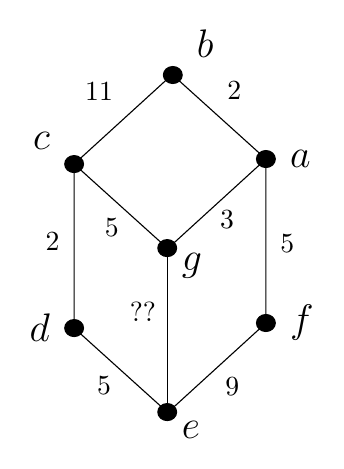
\begin{tikzpicture}[x=0.75pt,y=0.75pt,yscale=-1,xscale=1]
    %uncomment if require: \path (0,244); %set diagram left start at 0, and has height of 244
    
    %Shape: Cube [id:dp6646435130858394] 
    \draw   (39.45,81.85) -- (86.73,38.72) -- (131.84,79.43) -- (131.84,158.44) -- (84.55,201.57) -- (39.45,160.85) -- cycle ; \draw   (131.84,79.43) -- (84.55,122.56) -- (39.45,81.85) ; \draw   (84.55,122.56) -- (84.55,201.57) ;
    %Shape: Ellipse [id:dp7053935929182301] 
    \draw  [fill={rgb, 255:red, 0; green, 0; blue, 0 }  ,fill opacity=1 ] (82.46,38.95) .. controls (82.46,36.69) and (84.49,34.86) .. (86.99,34.86) .. controls (89.49,34.86) and (91.52,36.69) .. (91.52,38.95) .. controls (91.52,41.2) and (89.49,43.03) .. (86.99,43.03) .. controls (84.49,43.03) and (82.46,41.2) .. (82.46,38.95) -- cycle ;
    %Shape: Ellipse [id:dp3846430227043952] 
    \draw  [fill={rgb, 255:red, 0; green, 0; blue, 0 }  ,fill opacity=1 ] (127.31,79.42) .. controls (127.31,77.17) and (129.34,75.34) .. (131.84,75.34) .. controls (134.34,75.34) and (136.37,77.17) .. (136.37,79.42) .. controls (136.37,81.68) and (134.34,83.51) .. (131.84,83.51) .. controls (129.34,83.51) and (127.31,81.68) .. (127.31,79.42) -- cycle ;
    %Shape: Ellipse [id:dp3122259521210028] 
    \draw  [fill={rgb, 255:red, 0; green, 0; blue, 0 }  ,fill opacity=1 ] (79.77,122.33) .. controls (79.77,120.07) and (81.79,118.25) .. (84.29,118.25) .. controls (86.8,118.25) and (88.82,120.07) .. (88.82,122.33) .. controls (88.82,124.59) and (86.8,126.42) .. (84.29,126.42) .. controls (81.79,126.42) and (79.77,124.59) .. (79.77,122.33) -- cycle ;
    %Shape: Ellipse [id:dp5568900450079106] 
    \draw  [fill={rgb, 255:red, 0; green, 0; blue, 0 }  ,fill opacity=1 ] (34.92,81.86) .. controls (34.92,79.6) and (36.95,77.77) .. (39.45,77.77) .. controls (41.95,77.77) and (43.97,79.6) .. (43.97,81.86) .. controls (43.97,84.11) and (41.95,85.94) .. (39.45,85.94) .. controls (36.95,85.94) and (34.92,84.11) .. (34.92,81.86) -- cycle ;
    %Shape: Ellipse [id:dp5276475452889409] 
    \draw  [fill={rgb, 255:red, 0; green, 0; blue, 0 }  ,fill opacity=1 ] (34.92,160.86) .. controls (34.92,158.61) and (36.95,156.78) .. (39.45,156.78) .. controls (41.95,156.78) and (43.97,158.61) .. (43.97,160.86) .. controls (43.97,163.12) and (41.95,164.95) .. (39.45,164.95) .. controls (36.95,164.95) and (34.92,163.12) .. (34.92,160.86) -- cycle ;
    %Shape: Ellipse [id:dp01895932765963071] 
    \draw  [fill={rgb, 255:red, 0; green, 0; blue, 0 }  ,fill opacity=1 ] (79.77,201.34) .. controls (79.77,199.08) and (81.79,197.25) .. (84.29,197.25) .. controls (86.8,197.25) and (88.82,199.08) .. (88.82,201.34) .. controls (88.82,203.6) and (86.8,205.43) .. (84.29,205.43) .. controls (81.79,205.43) and (79.77,203.6) .. (79.77,201.34) -- cycle ;
    %Shape: Ellipse [id:dp8485087793178528] 
    \draw  [fill={rgb, 255:red, 0; green, 0; blue, 0 }  ,fill opacity=1 ] (127.31,158.43) .. controls (127.31,156.17) and (129.34,154.34) .. (131.84,154.34) .. controls (134.34,154.34) and (136.37,156.17) .. (136.37,158.43) .. controls (136.37,160.69) and (134.34,162.52) .. (131.84,162.52) .. controls (129.34,162.52) and (127.31,160.69) .. (127.31,158.43) -- cycle ;
    
    % Text Node
    \draw (142.19,79.42) node [anchor=west] [inner sep=0.75pt]  [font=\Large]  {$a$};
    % Text Node
    \draw (97.34,31.74) node [anchor=south west] [inner sep=0.75pt]  [font=\Large]  {$b$};
    % Text Node
    \draw (29.1,76.02) node [anchor=south east] [inner sep=0.75pt]  [font=\Large]  {$c$};
    % Text Node
    \draw (29.1,160.86) node [anchor=east] [inner sep=0.75pt]  [font=\Large]  {$d$};
    % Text Node
    \draw (90.12,204.46) node [anchor=north west][inner sep=0.75pt]  [font=\Large]  {$e$};
    % Text Node
    \draw (142.19,158.43) node [anchor=west] [inner sep=0.75pt]  [font=\Large]  {$f$};
    % Text Node
    \draw (90.12,123.54) node [anchor=north west][inner sep=0.75pt]  [font=\Large]  {$g$};
    % Text Node
    \draw (112,40.9) node [anchor=north west][inner sep=0.75pt]    {$2$};
    % Text Node
    \draw (108.5,102.9) node [anchor=north west][inner sep=0.75pt]    {$3$};
    % Text Node
    \draw (137.5,114.4) node [anchor=north west][inner sep=0.75pt]    {$5$};
    % Text Node
    \draw (58.44,182.9) node [anchor=north east] [inner sep=0.75pt]    {$5$};
    % Text Node
    \draw (24.5,113.4) node [anchor=north west][inner sep=0.75pt]    {$2$};
    % Text Node
    \draw (43.5,41.4) node [anchor=north west][inner sep=0.75pt]    {$11$};
    % Text Node
    \draw (111,183.4) node [anchor=north west][inner sep=0.75pt]    {$9$};
    % Text Node
    \draw (53,106.9) node [anchor=north west][inner sep=0.75pt]    {$5$};
    % Text Node
    \draw (65,147.4) node [anchor=north west][inner sep=0.75pt]    {$??$};
    
    
    \end{tikzpicture}
    

    
\end{figure}

\begin{enumerate}
    \item \label{firstQnSec1} Write down the list of vertices of $G$: (4 points)
    \vspace{0.5em}
    $$V=\left\lbrace\hspace{7.5cm}\right\rbrace.$$
    \vfill
    \item Write down the list of edges of $G$: (4 points)
    \vspace{0.5em}
    $$E=\left\lbrace\hspace{10cm}\right\rbrace.$$
    \vfill
    \item Out of the following, which is \textbf{NOT} an edge in the graph? (2 points)
    \begin{checkboxes}
        \choice $ag$
        \choice $dg$
        \choice $ef$
        \choice $bc$
    \end{checkboxes}
    \vfill
    \item How many vertices does this graph have? (2 points)
    \begin{checkboxes}
        \choice 3
        \choice 6
        \choice 7
        \choice 8
    \end{checkboxes}
    \vfill
    \newpage
    \item The degrees of the vertices $d,e,f$ and $g$ respectively are: (2 points)
    \begin{checkboxes}
        \choice $5,6,7,8$
        \choice $1,2,3,4$
        \choice $2,3,2,3$
        \choice $6,7,6,7$
    \end{checkboxes}
    \vfill
    \item A path of length $3$ from $a$ to $d$ passing through $f$ is: (2 points)
    \begin{checkboxes}
        \choice $ab,bc,cd$
        \choice $ag,gc,cd$
        \choice $ag,ge,ed$
        \choice $af,fe,ed$
    \end{checkboxes}
    \vfill
    \item Does this graph have cut-edges? (2 points)
    \begin{checkboxes}
        \choice Yes.
        \choice No.
    \end{checkboxes}
    \vfill
    \item State whether this graph has an Euler tour. If it does, write it down, if not state why it doesn't. (2 points)
    \vspace{7em}
    \vfill
    \item State whether this graph has an Hamilton tour. If it does, write it down, if not state why it doesn't. (2 points)
    \vspace{7em}
    \vfill
    \item The graph $G$ doesn't have an Euler circuit, Eulerize it by adding edges: (2 points)
    \begin{figure}[h!]
        \centering
        \tikzset{every picture/.style={line width=0.75pt}} %set default line width to 0.75pt        
    
        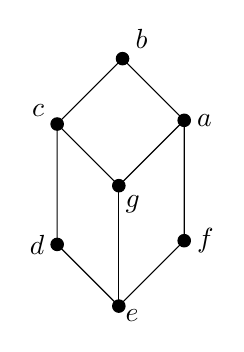
\begin{tikzpicture}[x=0.75pt,y=0.75pt,yscale=-1,xscale=1]
        %uncomment if require: \path (0,300); %set diagram left start at 0, and has height of 300
        
        %Shape: Cube [id:dp6646435130858394] 
        \draw   (30.79,59.04) -- (62.29,27.54) -- (92,57.25) -- (92,115.25) -- (60.5,146.75) -- (30.79,117.04) -- cycle ; \draw   (92,57.25) -- (60.5,88.75) -- (30.79,59.04) ; \draw   (60.5,88.75) -- (60.5,146.75) ;
        %Shape: Circle [id:dp7053935929182301] 
        \draw  [fill={rgb, 255:red, 0; green, 0; blue, 0 }  ,fill opacity=1 ] (59.29,27.54) .. controls (59.29,25.88) and (60.63,24.54) .. (62.29,24.54) .. controls (63.94,24.54) and (65.29,25.88) .. (65.29,27.54) .. controls (65.29,29.19) and (63.94,30.54) .. (62.29,30.54) .. controls (60.63,30.54) and (59.29,29.19) .. (59.29,27.54) -- cycle ;
        %Shape: Circle [id:dp3846430227043952] 
        \draw  [fill={rgb, 255:red, 0; green, 0; blue, 0 }  ,fill opacity=1 ] (89,57.25) .. controls (89,55.59) and (90.34,54.25) .. (92,54.25) .. controls (93.66,54.25) and (95,55.59) .. (95,57.25) .. controls (95,58.91) and (93.66,60.25) .. (92,60.25) .. controls (90.34,60.25) and (89,58.91) .. (89,57.25) -- cycle ;
        %Shape: Circle [id:dp3122259521210028] 
        \draw  [fill={rgb, 255:red, 0; green, 0; blue, 0 }  ,fill opacity=1 ] (57.5,88.75) .. controls (57.5,87.09) and (58.84,85.75) .. (60.5,85.75) .. controls (62.16,85.75) and (63.5,87.09) .. (63.5,88.75) .. controls (63.5,90.41) and (62.16,91.75) .. (60.5,91.75) .. controls (58.84,91.75) and (57.5,90.41) .. (57.5,88.75) -- cycle ;
        %Shape: Circle [id:dp5568900450079106] 
        \draw  [fill={rgb, 255:red, 0; green, 0; blue, 0 }  ,fill opacity=1 ] (27.79,59.04) .. controls (27.79,57.38) and (29.13,56.04) .. (30.79,56.04) .. controls (32.44,56.04) and (33.79,57.38) .. (33.79,59.04) .. controls (33.79,60.69) and (32.44,62.04) .. (30.79,62.04) .. controls (29.13,62.04) and (27.79,60.69) .. (27.79,59.04) -- cycle ;
        %Shape: Circle [id:dp5276475452889409] 
        \draw  [fill={rgb, 255:red, 0; green, 0; blue, 0 }  ,fill opacity=1 ] (27.79,117.04) .. controls (27.79,115.38) and (29.13,114.04) .. (30.79,114.04) .. controls (32.44,114.04) and (33.79,115.38) .. (33.79,117.04) .. controls (33.79,118.69) and (32.44,120.04) .. (30.79,120.04) .. controls (29.13,120.04) and (27.79,118.69) .. (27.79,117.04) -- cycle ;
        %Shape: Circle [id:dp01895932765963071] 
        \draw  [fill={rgb, 255:red, 0; green, 0; blue, 0 }  ,fill opacity=1 ] (57.5,146.75) .. controls (57.5,145.09) and (58.84,143.75) .. (60.5,143.75) .. controls (62.16,143.75) and (63.5,145.09) .. (63.5,146.75) .. controls (63.5,148.41) and (62.16,149.75) .. (60.5,149.75) .. controls (58.84,149.75) and (57.5,148.41) .. (57.5,146.75) -- cycle ;
        %Shape: Circle [id:dp8485087793178528] 
        \draw  [fill={rgb, 255:red, 0; green, 0; blue, 0 }  ,fill opacity=1 ] (89,115.25) .. controls (89,113.59) and (90.34,112.25) .. (92,112.25) .. controls (93.66,112.25) and (95,113.59) .. (95,115.25) .. controls (95,116.91) and (93.66,118.25) .. (92,118.25) .. controls (90.34,118.25) and (89,116.91) .. (89,115.25) -- cycle ;
        
        % Text Node
        \draw (97,57.25) node [anchor=west] [inner sep=0.75pt]    {$a$};
        % Text Node
        \draw (67.29,24.14) node [anchor=south west] [inner sep=0.75pt]    {$b$};
        % Text Node
        \draw (25.79,56.64) node [anchor=south east] [inner sep=0.75pt]    {$c$};
        % Text Node
        \draw (25.79,117.04) node [anchor=east] [inner sep=0.75pt]    {$d$};
        % Text Node
        \draw (62.5,147.15) node [anchor=north west][inner sep=0.75pt]    {$e$};
        % Text Node
        \draw (97,115.25) node [anchor=west] [inner sep=0.75pt]    {$f$};
        % Text Node
        \draw (62.5,92.15) node [anchor=north west][inner sep=0.75pt]    {$g$};
        
        
        \end{tikzpicture}
        
    \end{figure}
    \vfill 
    \item \label{lastQnSec1} State whether this graph has an Hamilton tour. If it does, write it down, if not state why it doesn't. (2 points)
    \vspace{7em}
    \vfill
\end{enumerate}
\item For questions \ref{firstQnSec2} through \ref{lastQnSec2} consider the information about the graph $G$ given by the following lists:
\begin{gather*}
    V=\left\lbrace a,b,c,d,e,f\right\rbrace\\
    E=\left\lbrace ad,ae,bc,bd,cd,cf,de,df,ef\right\rbrace\\
\end{gather*}
\begin{enumerate}
\item \label{firstQnSec2} Fill in the edges of the graph $G$: (4 points)
\begin{figure}[h!]
    \centering
    \tikzset{every picture/.style={line width=0.75pt}} %set default line width to 0.75pt        

    \begin{tikzpicture}[x=0.75pt,y=0.75pt,yscale=-1,xscale=1]
    %uncomment if require: \path (0,300); %set diagram left start at 0, and has height of 300
    
    %Shape: Circle [id:dp24175619248880365] 
    \draw  [fill={rgb, 255:red, 0; green, 0; blue, 0 }  ,fill opacity=1 ] (195.88,124.87) .. controls (195.88,122.67) and (197.67,120.87) .. (199.88,120.87) .. controls (202.08,120.87) and (203.88,122.67) .. (203.88,124.87) .. controls (203.88,127.08) and (202.08,128.87) .. (199.88,128.87) .. controls (197.67,128.87) and (195.88,127.08) .. (195.88,124.87) -- cycle ;
    %Shape: Circle [id:dp38562246159096747] 
    \draw  [fill={rgb, 255:red, 0; green, 0; blue, 0 }  ,fill opacity=1 ] (158.5,60.05) .. controls (158.5,57.84) and (160.29,56.05) .. (162.5,56.05) .. controls (164.71,56.05) and (166.5,57.84) .. (166.5,60.05) .. controls (166.5,62.26) and (164.71,64.05) .. (162.5,64.05) .. controls (160.29,64.05) and (158.5,62.26) .. (158.5,60.05) -- cycle ;
    %Shape: Circle [id:dp9956752087587961] 
    \draw  [fill={rgb, 255:red, 0; green, 0; blue, 0 }  ,fill opacity=1 ] (83.5,60.05) .. controls (83.5,57.84) and (85.29,56.05) .. (87.5,56.05) .. controls (89.71,56.05) and (91.5,57.84) .. (91.5,60.05) .. controls (91.5,62.26) and (89.71,64.05) .. (87.5,64.05) .. controls (85.29,64.05) and (83.5,62.26) .. (83.5,60.05) -- cycle ;
    %Shape: Circle [id:dp24033698556569782] 
    \draw  [fill={rgb, 255:red, 0; green, 0; blue, 0 }  ,fill opacity=1 ] (46,125) .. controls (46,122.79) and (47.79,121) .. (50,121) .. controls (52.21,121) and (54,122.79) .. (54,125) .. controls (54,127.21) and (52.21,129) .. (50,129) .. controls (47.79,129) and (46,127.21) .. (46,125) -- cycle ;
    %Shape: Circle [id:dp10560264310320788] 
    \draw  [fill={rgb, 255:red, 0; green, 0; blue, 0 }  ,fill opacity=1 ] (83.5,189.95) .. controls (83.5,187.74) and (85.29,185.95) .. (87.5,185.95) .. controls (89.71,185.95) and (91.5,187.74) .. (91.5,189.95) .. controls (91.5,192.16) and (89.71,193.95) .. (87.5,193.95) .. controls (85.29,193.95) and (83.5,192.16) .. (83.5,189.95) -- cycle ;
    %Shape: Circle [id:dp03400871765845248] 
    \draw  [fill={rgb, 255:red, 0; green, 0; blue, 0 }  ,fill opacity=1 ] (158.5,189.95) .. controls (158.5,187.74) and (160.29,185.95) .. (162.5,185.95) .. controls (164.71,185.95) and (166.5,187.74) .. (166.5,189.95) .. controls (166.5,192.16) and (164.71,193.95) .. (162.5,193.95) .. controls (160.29,193.95) and (158.5,192.16) .. (158.5,189.95) -- cycle ;
    
    % Text Node
    \draw (165.31,53.16) node [anchor=south west] [inner sep=0.75pt]  [font=\Large]  {$a$};
    % Text Node
    \draw (85.5,56.65) node [anchor=south east] [inner sep=0.75pt]  [font=\LARGE]  {$b$};
    % Text Node
    \draw (41,120) node [anchor=east] [inner sep=0.75pt]  [font=\LARGE]  {$c$};
    % Text Node
    \draw (85.5,193.35) node [anchor=north east] [inner sep=0.75pt]  [font=\LARGE]  {$d$};
    % Text Node
    \draw (205.88,124.87) node [anchor=west] [inner sep=0.75pt]  [font=\LARGE]  {$f$};
    % Text Node
    \draw (164.5,201.35) node [anchor=north west][inner sep=0.75pt]  [font=\LARGE]  {$e$};
    
    
    \end{tikzpicture}
    
    


\end{figure}
\vfill
\item List all the vertices adjacent to $d$: (2 points)
$$N(d)=\left\lbrace\hspace{7cm}\right\rbrace$$
\vfill
\item What is the degree of the vertex $d$? (2 points)
$$\deg(d)=\hspace{3cm}$$
\vfill
\item Find the sum of the degrees of all vertices: (2 points)
\begin{checkboxes}
    \choice 6
    \choice 9
    \choice 12
    \choice 18
\end{checkboxes}
\vfill
\item State whether this graph has an Euler tour. If it does, write it down, if not state why it doesn't. (2 points)
    \vspace{7em}
\vfill
\item State whether this graph has an Euler circuit. If it does, write it down, if not Eulerize it. (2 points)
    \vspace{7em}
\vfill
\item \label{lastQnSec2} For the previous value, which players have veto power, why? (2 points)
\begin{checkboxes}
    \choice Both Natalie and Oscar have veto power because all motions can pass without their consideration.
    \choice (CORRECT) Both Markus and Natalie have veto power because no motion can pass without both of their votes.
    \choice Both Oscar and Pauline have veto power because no coalition can pass any motion at all.
    \choice Both Natalie and Pauline have veto power because they need the support of all the players to pass a motion.
\end{checkboxes}
\vfill
\end{enumerate}
\newpage

\item In this exercise we will explore graphs with Euler and Hamilton walks or circuits. Follow the instructions and complete each task as asked:
\begin{itemize}
    \item Explain the difference between a walk and a circuit of a graph. (4 points)
    \item Explain the difference between Eulerian and Hamiltonian paths or circuits. (4 points)
    \item Draw a graph (doesn't need to be very big) which contains an Euler tour but not an Euler circuit. (4 points)
    \item Draw a graph which contains a Hamilton tour but doesn't have an Euler tour. (4 points)
    \item Draw a graph which contains an Euler circuit but not a Hamilton tour. (4 points)
    \item Extra: ¿Can you draw a graph with an Euler circuit and a Hamilton tour but not a Hamilton circuit? (4 extra points)
    \item Extra: ¿Can you draw a graph with an Euler tour and a Hamilton circuit but not a Euler circuit? (4 extra points)
\end{itemize}


Sol:
\begin{enumerate}
    \item A walk starts and ends at different places whereas a circuit begins and ends at the same place.
    \item Eulerian means that edges are the object of interest to traverse, while Hamiltonian means that the vertices are the traversed ones.
    \item Any path graph.
    \item A path graph with any pair of middle vertices connected.
    \item Two triangles joined at a vertex, say a ribbon.
    \item The ribbon graph again.
    \item A cycle with more than four vertices with any two non-adjacent vertices connected.
\end{enumerate}


\end{enumerate}
\end{document}

